% -- Encoding UTF-8 without BOM
% -- XeLaTeX => PDF (BIBER)

\documentclass[espanol]{cv-style}          % Add 'print' as an option into the square bracket to remove colours from this template for printing. 
                                    % Add 'espanol' as an option into the square bracket to change the date format of the Last Updated Text
\usepackage[spanish]{babel} 
%\sethyphenation[]{spanish} % Add words between the {} to avoid them to be cut 
\usepackage{graphicx}
\begin{document}

\header{Rafael de Moura }{Moreira}           % Your name
\lastupdated

%----------------------------------------------------------------------------------------
%	SIDEBAR SECTION  -- In the aside, each new line forces a line break
%----------------------------------------------------------------------------------------

\begin{aside}
\section{.}
\flushleft%
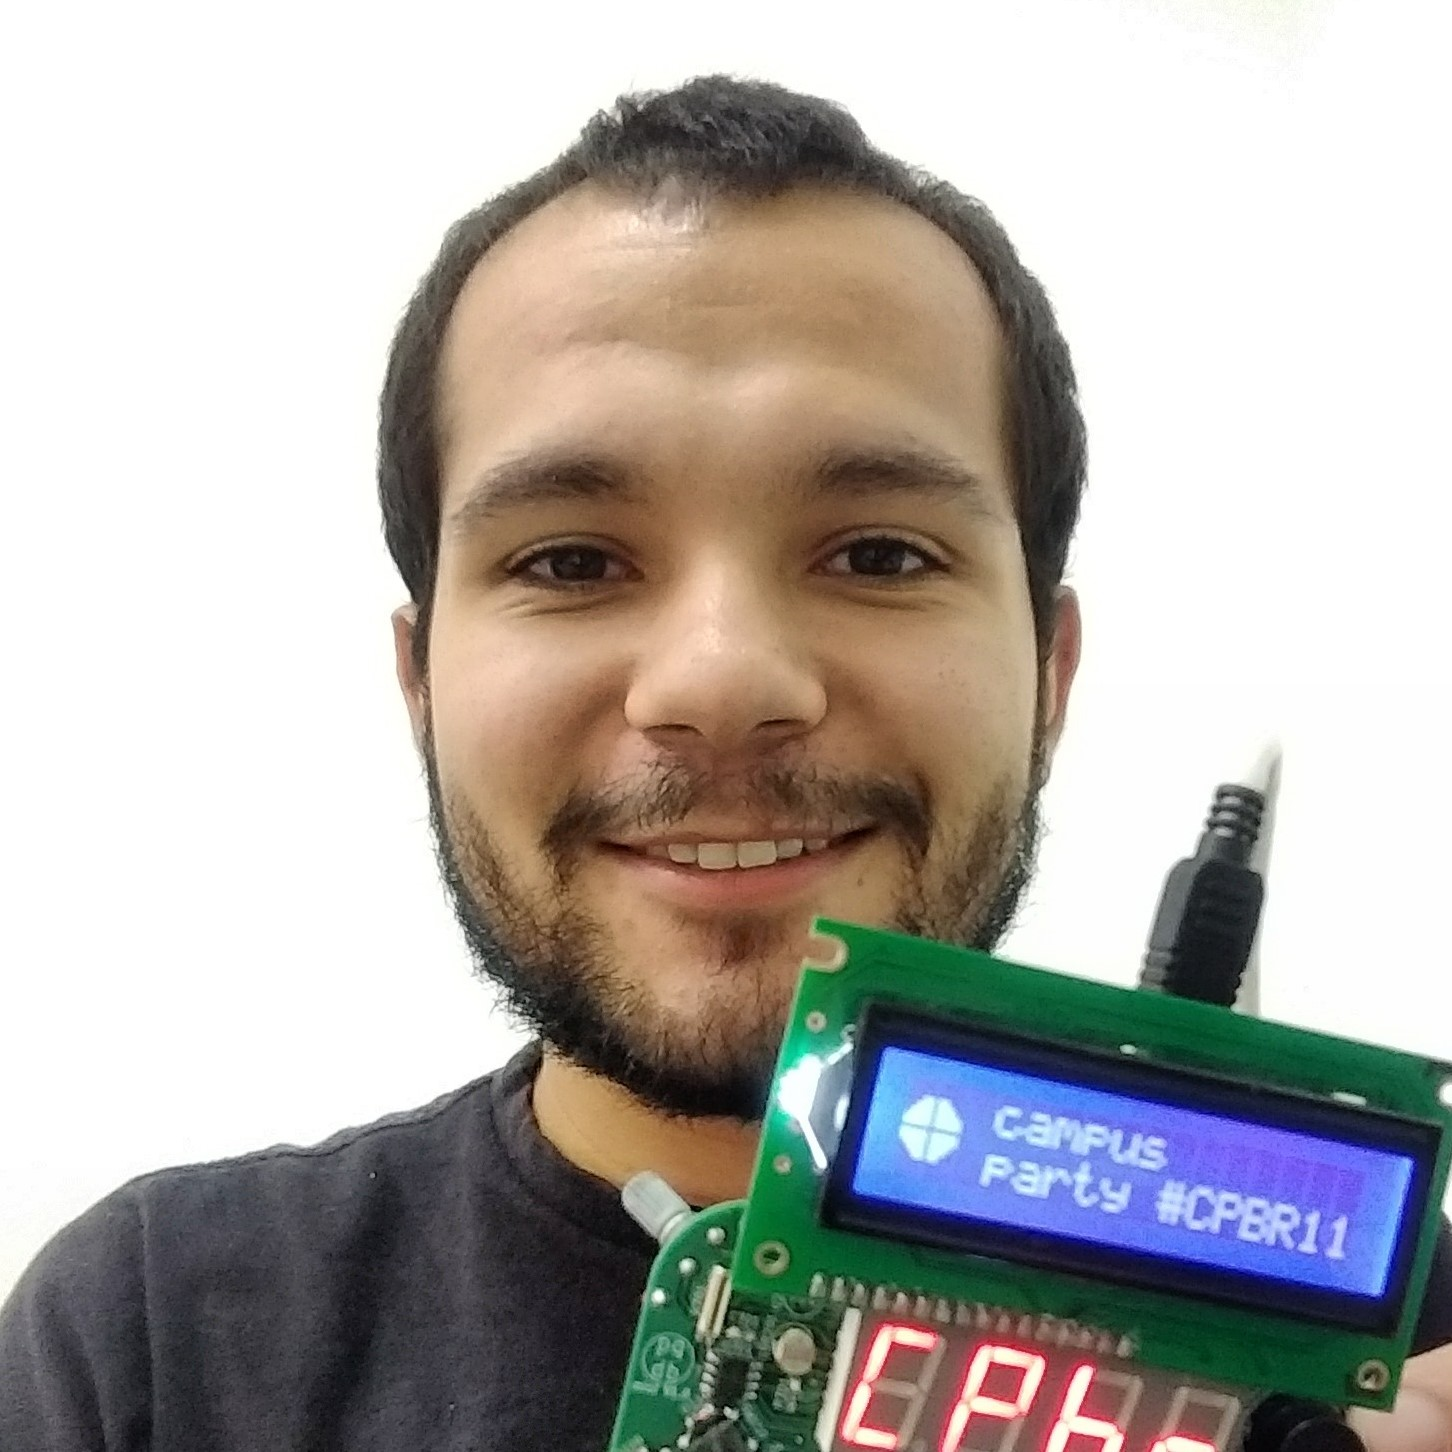
\includegraphics[width=4cm]{photo}
\section{Contacto}
\href{https://wa.me/5511945545955}{+55 11 94554-5955}
~
\href{mailto:rafaelmmoreira@gmail.com}{rafaelmmoreira@gmail.com}
~
\url{https://www.linkedin.com/in/rafaelmmoreira/}
~
\url{https://github.com/rafaelmmoreira/}
%
\section{Idiomas}
Portugués: nativo
Inglés: fluido
Espanhol: avanzado
Francês: principiante
%
\section{Intereses profesionales}
Desarrollo de software
Prototipado de hardware
Análisis de datos
Enseñanza y divulgación de las ciências e tecnología
%
\vspace{3.7cm}
Versión más reciente:

\includegraphics[width=4cm]{qrcode}
Available in English.
Disponível em Português.
%
\end{aside}

%----------------------------------------------------------------------------------------
%	SKILLS SECTION
%----------------------------------------------------------------------------------------

\section{Educación}
\vspace{-0.3cm}
\begin{entrylist}
\entry
{}
{\textbf{Maestría en Ciencia y Tecnología de Computación}}
{}
{\textit{ Universidade Federal de Itajubá, 2019.}}
{}

\entry
{}
{\textbf{ Licenciatura en Ingeneria en Computación }}
{}
{\textit{ Universidade Federal de Itajubá, 2015.}}
{}

\entry
{}
{\textbf{Especialización (posgrado) en Data Science}}
{}
{\textit{Centro Universitário Faculdades Metropolitanas Unidas (en progreso).}}
{}

\entry
{}
{\textbf{Especialización (posgrado)  en Desarrolamiento de Software con Metodologías Ágiles}}
{}
{\textit{Universidade Anhembi Morumbi (en progreso).}}
{}

\end{entrylist}
{\vspace{-0.8cm}}
%	WORK EXPERIENCE SECTION
%----------------------------------------------------------------------------------------

\section{Experiencia profesional}
\vspace{-0.3cm}
\begin{entrylist}
%------------------------------------------------


%----------------------------------------------------------------------------------------
\entry
{}
{Analista-programador | Setis (PayGo/C6 Bank) | oct/18 - presente}
{\vspace{-0.01cm}}
{Desarrollo de software embebido para diversos terminales POS (dispositivos de tarjeta de crédito) para una gran adquirente brasileña en lenguaje C y metodología Scrum. Automación de procesos de creacion de paquetes con Python.}
{}
 %----------------------------------------------------------------------------------------

\entry
  {}
  {Maestro de programación | Let's Code Academy | ene/19 - presente}
  {\vspace{-0.01cm}}
{Maestro del curso Python Pro (algoritmos, estructuras de datos, programación orientada a objetos, interfaz de usuario, obtener datos de APIs y webscraping). Escrita de un libro de Python y de un capítulo sobre visualización de datos para un libro de Data Science.}
 {} %----------------------------------------------------------------------------------------

\entry
  {}
  {Profesor temporario | Universidade Federal de Itajubá | feb/17 - oct/18}
{\vspace{-0.01cm}}
{ Maestro de lógica de programación en los grados de Ingeneria en Computación, Electrónica y en Automatización y Control. Lenguajes C y Python. Coordinador de los proyectos Dev-U (equipo de programación de videojuegos) y ProgramAção (equipo de enseñantes de programación para adolescentes).}
 %----------------------------------------------------------------------------------------
\end{entrylist}
{\vspace{-0.4cm}}

\section{Palestras y conferencias}
\vspace{-0.3cm}
\begin{entrylist}

\entry
{}
{Algunas conferencias y cursos impartidos (todos en Portugués):}
{}
{\vspace{-0.5cm}}

%------------------------------------------------
\entry
{}
{\href{https://www.slideshare.net/rafaelmmoreira/como-fazer-seu-prprio-gameboy-cpbr11}{Como hacer tu propio Gameboy}}
{\href{https://campuse.ro/events/campus-party-brasil-2018/workshop/como-fazer-seu-proprio-gameboy-cpbr11/}{Campus Party Brasil, 2018}}
{\vspace{-0.5cm}}
%------------------------------------------------
\entry
{}
{\href{https://www.slideshare.net/rafaelmmoreira/desenvolvimento-de-sistemas-embarcados-do-hardware-ao-software}{Desarrollo de sistemas embebidos}}
{\href{https://sp13.securitybsides.com.br/detalhe-dos-treinamentos-e-apresentacoes/}{BSides São Paulo, 2016}}
{\vspace{-0.5cm}}
%------------------------------------------------
\entry
{}
{\href{https://www.slideshare.net/rafaelmmoreira/escalonador-earliest-deadline-first-tdc2014sp}{Planificador Earliest Deadline First}}
{\href{https://thedevconf.com/tdc/2014/saopaulo/trilha-embedded}{The Developer's Conference São Paulo, 2014}}
{\vspace{-0.5cm}}
%------------------------------------------------
\entry
{}
{\href{https://www.slideshare.net/rafaelmmoreira/programao-segura}{Programación segura}}
{\href{https://garoa.net.br/wiki/O_Outro_Lado_BSidesSP_ed_naovaitercopa/Lightning_Talks}{BSides São Paulo, 2014}}
{\vspace{-0.5cm}}
%------------------------------------------------

%------------------------------------------------
\end{entrylist}
{\vspace{-0.2cm}}
%-------------------------------  ---------------------------------------------------------
%	END HOBBIES SECTION SECTION

\section{Artículos publicados}
\vspace{-0.3cm}
\begin{entrylist}
%------------------------------------------------
\entry
{}
{}
{\vspace{-0.4cm}}
{\href{https://doi.org/10.1109/ICM48031.2019.9021277}{MOREIRA, R. M. et al. \textbf{Online Heartbeat Classification Using Low Cost Algorithms}. In: 31st INTERNATIONAL CONFERENCE ON MICROELECTRONICS (IEEE-ICM), 2019, Cairo, Egito.}}
{}
%------------------------------------------------
\entry
{}
{}
{\vspace{-0.01cm}}
{\href{http://www.swge.inf.br/CBA2014/anais/PDF/1569927865.pdf}{MOREIRA, R. M. et al. \textbf{Plataforma Didática de Baixo Custo para Experiências em Laboratórios de Controle}. In: XX CONGRESSO BRASILEIRO DE AUTOMÁTICA, 2014, Belo Horizonte.}}
{}
\end{entrylist}
{\vspace{-0.4cm}}

%%%%%%%%%
\section{Lenguajes y herramientas}
\vspace{-0.3cm}
\begin{entrylist}
\entry
{}
{Lenguajes de programación más utilizadas:}
{C, Python}
{\vspace{-0.5cm}}
\entry
{}
{Herramientas de modelos y análisis de datos}
{Anaconda (Python), MATLAB, Octave}
{\vspace{-0.5cm}}
\entry
{}
{Microcontroladores y placas embebidas}
{Arduino, Raspberry Pi, HCS12, PIC18F}
{\vspace{-0.5cm}}
\entry
{}
{Metodologías de desarrollo ágil}
{Scrum, XP}
{\vspace{-0.5cm}}
\entry
{}
{Versionado de software}
{GitHub}
{\vspace{-0.5cm}}
\entry
{}
{Diferentes niveles de experiencia con otras lenguajes y facilidad para aprender nuevas herramientas. }
{}
{\vspace{-4.0cm}}
\end{entrylist}


\end{document}
